\begin{name}
	{\tenchude}{\tendethi}{LỚP TOÁN THẦY PHÁT}{\thoigian}
\end{name}
\setcounter{ex}{0}\setcounter{bt}{0}
\Opensolutionfile{ans}[ans/ans-2-TT-27-Lientruong-NgheAn-23]
\begin{ex}%[Thi thử tốt nghiệp - Liên trường THPT Nghệ An - 23]%[Huỳnh Xuân Tín - EX6]%[2H1Y3-2]
	Cho khối lăng trụ có chiều cao bằng $6$ và diện tích đáy bằng $10$. Tính thể tích khối lăng trụ đó.	
	\choice
	{$600$}
	{\True $60$}
	{$20$}
	{$360$}
	\loigiai{
		Thể tích khối lăng trụ có chiều cao bằng $6$ và diện tích đáy bằng $10$ là $V=6\cdot 10=60$.
	}
\end{ex}
\begin{ex}%[Thi thử tốt nghiệp - Liên trường THPT Nghệ An - 23]%[Huỳnh Xuân Tín - EX6]%[2D1Y2-2]
	Cho hàm số $y=f(x)$ có bảng biến thiên như sau
	\begin{center}
		
\begin{tikzpicture}
			\tkzTabInit[nocadre=false,lgt=1.2,espcl=2.5,deltacl=0.6]
			{$x$ /0.6, $y'$ /0.6, $y$ /2.5}
			{$-\infty$,$0$,$2$,$+\infty$}
			\tkzTabLine{,-,$0$,+,$0$,-,}
			\tkzTabVar{+/$+\infty$,-/$1$,+/$5$,-/$-\infty$}
		\end{tikzpicture}
	\end{center}	
	Điểm cực tiểu của hàm số là
	\choice
	{$x=2$}
	{$x=5$}
	{\True $x=0$}
	{ $x=1$}
	\loigiai{
		Từ bảng biến thiên trên ta suy ra điểm cực tiểu của hàm số là $x=0$.		
	}
\end{ex}
\begin{ex}%[Thi thử tốt nghiệp - Liên trường THPT Nghệ An - 23]%[Huỳnh Xuân Tín - EX6]%[2D1Y1-2]
	Cho hàm số $y=f(x)$ có bảng xét dấu đạo hàm như sau
	\begin{center}
		
\begin{tikzpicture}
			\tkzTabInit[nocadre=false,lgt=1.2,espcl=2.5,deltacl=0.6]
			{$x$ /0.6, $f'(x)$ /0.6}
			{$-\infty$,$-1$,$0$,$1$,$+\infty$}
			\tkzTabLine{,-,$0$,+,$0$,-,$0$,+,}
		\end{tikzpicture}
	\end{center}	
	Hàm số đã cho nghịch biến trên khoảng
	\choice
	{$(1;+\infty)$}
	{\True $(-2;-1)$}
	{$(-1;0)$}
	{$(-1;1)$}
	\loigiai{
		Từ bảng xét của $f'(x)$ ta suy ra hàm số đã cho nghịch biến trên các khoảng $(-\infty;-1)$, $(0;1)$.		
	}
\end{ex}
\begin{ex}%[Thi thử tốt nghiệp - Liên trường THPT Nghệ An - 23]%[Huỳnh Xuân Tín - EX6]%[2D2Y4-2]
	Trên khoảng $(1 ;+\infty)$, đạo hàm của hàm số $y=\log _5(x-1)$ là	
	\choice
	{$y'=\dfrac{\ln 5}{x-1}$}
	{$y'=-\dfrac{1}{(x-1) \ln 5}$}
	{$y'=\dfrac{1}{x-1}$}
	{\True $y'=\dfrac{1}{(x-1) \ln 5}$}
	\loigiai{
		Ta có 	$y'=\left(\log _5(x-1)\right)'=\dfrac{(x-1)'}{(x-1)\ln 5}=\dfrac{1}{(x-1)\ln 5}$.	
	}
\end{ex}
\begin{ex}%[Thi thử tốt nghiệp - Liên trường THPT Nghệ An - 23]%[Huỳnh Xuân Tín - EX6]%[2H2Y1-2]
	Cho hình trụ có bán kính đáy bằng $r$ và chiều cao bằng $h$. Tính diện tích toàn phần của hình trụ đó.	
	\choice
	{$\pi r^2h$}
	{\True $2\pi r(r+h)$}
	{$2\pi rh$}
	{$\pi rh$}
	\loigiai{
		Diện tích toàn phần của hình trụ có bán kính đáy bằng $r$ và chiều cao bằng $h$ là
		\[2\pi rh+2\pi r^2=2\pi r(r+h).\]	
	}
\end{ex}
\begin{ex}%[Thi thử tốt nghiệp - Liên trường THPT Nghệ An - 23]%[Huỳnh Xuân Tín - EX6]%[2D2Y6-1]
	Tập nghiệm của bất phương trình $4^{x+1}<16$ là	
	\choice
	{$(1;+\infty)$}
	{$[1 ;+\infty)$}
	{\True $(-\infty;1)$}
	{$(-\infty ; 1]$}
	\loigiai{
		Ta có 	$4^{x+1}<16\Leftrightarrow x+1<2\Leftrightarrow x<1$.\\
		Vậy tập nghiệm của bất phương trình đã cho là $(-\infty;1)$.	
	}
\end{ex}
\begin{ex}%[Thi thử tốt nghiệp - Liên trường THPT Nghệ An - 23]%[Huỳnh Xuân Tín - EX6]%[2D1Y5-1]
	\immini{Đường cong trong hình dưới đây là đồ thị của hàm số nào trong các hàm số sau?	\choice
		{$y=x^3-3x+4$}
		{\True $y=-x^3-3x^2+4$}
		{$y=x^4+2x^2$}
		{ $y=\dfrac{2x+1}{x+1}$}}{
		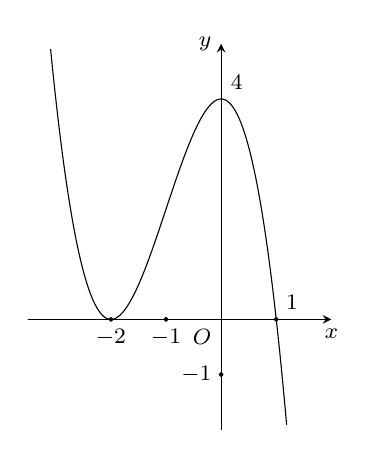
\begin{tikzpicture}[scale=0.7,>=stealth, font=\footnotesize, line join=round, line cap=round]
			\def\a{-1} \def\b{-3} \def\c{0} \def\d{4} % Hệ số
			\def\xmin{-3.5} \def\xmax{2}
			\def\ymin{-2} \def\ymax{5} 
			%	\draw[color=gray!50,dashed] (\xmin,\ymin) grid (\xmax,\ymax); 
			\draw[->] (\xmin,0)--(\xmax,0) node [below]{$x$};
			\draw[->] (0,\ymin)--(0,\ymax) node [left]{$y$};
			\node at (0,0) [below left]{$O$};
			\clip (\xmin+0.1,\ymin+0.1) rectangle (\xmax-0.5,\ymax-0.1);
			\draw[smooth,samples=300] plot(\x,{\a*(\x)^3+\b*(\x)^2+\c*(\x)+\d});
			\draw[fill=black] (-1,0) node[below]{$-1$} circle(1pt) (1,0) node[above right]{$1$}circle(1pt) (0,-1) circle(1pt) node[left]{$-1$} (0,4) node[above right]{$4$} (-2,0) node[below]{$-2$} circle(1pt);
	\end{tikzpicture}}	
	\loigiai{
		Dáng điệu của đồ thị trên là của hàm số bậc ba với hệ số cao nhất âm nên đó là đồ thị của hàm số 	$y=-x^3-3x^2+4$.	
	}
\end{ex}
\begin{ex}%[Thi thử tốt nghiệp - Liên trường THPT Nghệ An - 23]%[Huỳnh Xuân Tín - EX6]%[2D4Y1-1]
	Phần ảo của số phức $z=5-7 i$ là	
	\choice
	{$7$}
	{$5$}
	{\True $-7$}
	{$-7i$}
	\loigiai{
		Phần ảo của số phức $z=5-7 i$ là $-7$	
	}
\end{ex}
\begin{ex}%[Thi thử tốt nghiệp - Liên trường THPT Nghệ An - 23]%[Huỳnh Xuân Tín - EX6]%[2H3Y3-3]
	Trong KG $Oxyz$, cho đường thẳng $d\colon \dfrac{x-2}{3}=\dfrac{y}{-1}=\dfrac{z+3}{-2}$. Điểm nào dưới đây thuộc $d$?	
	\choice
	{$N(3;-1;-2)$}
	{$M(5;-1;0)$}
	{$P(-2;0;3)$}
	{\True $Q(2;0;-3)$}
	\loigiai{
		Ta có đường thẳng $d\colon \dfrac{x-2}{3}=\dfrac{y}{-1}=\dfrac{z+3}{-2}$ đi qua điểm $Q(2;0;-3)$.		
	}
\end{ex}
\begin{ex}%[Thi thử tốt nghiệp - Liên trường THPT Nghệ An - 23]%[Huỳnh Xuân Tín - EX6]%[2D4Y1-1]
	Mô đun của số phức $z=3-2 i$ là	
	\choice
	{$5$}
	{\True $\sqrt{13}$}
	{$\sqrt{5}$}
	{$13$}
	\loigiai{
		Mô đun của số phức $z=3-2 i$ là	$|z|=\sqrt{3^2+2^2}=\sqrt{13}$.		
	}
\end{ex}
\begin{ex}%[Thi thử tốt nghiệp - Liên trường THPT Nghệ An - 23]%[Huỳnh Xuân Tín - EX6]%[2H3Y1-4]
	Trong không gian $O x y z$, cho mặt cầu $(S)\colon x^2+y^2+z^2+6 x-4 y-2 z-2=0$. Tâm của $(S)$ có tọa độ là	
	\choice
	{$(3;-2;-1)$}
	{\True $(-3;2;1)$}
	{$(-6;4;2)$}
	{$(6;-4;-2)$}
	\loigiai{
		Mặt cầu $(S)\colon x^2+y^2+z^2+6 x-4 y-2 z-2=0$ có tâm là $(-3;2;1)$.		
	}
\end{ex}
\begin{ex}%[Thi thử tốt nghiệp - Liên trường THPT Nghệ An - 23]%[Huỳnh Xuân Tín - EX6]%[2D1Y4-1]
	Đường tiệm cận ngang của đồ thị hàm số $y=\dfrac{3 x+1}{x-1}$ là	
	\choice
	{$y=-1$}
	{\True $y=3$}
	{$x=3$}
	{$x=1$}
	\loigiai{
		Hàm số 	$y=\dfrac{3 x+1}{x-1}$	có tập xác định là $\mathscr{D}=\mathbb{R}\setminus\{1\}$ và có
		\[\lim\limits_{x\to +\infty}y=\lim\limits_{x\to +\infty}\dfrac{3 x+1}{x-1}=3, \lim\limits_{x\to -\infty}y=\lim\limits_{x\to -\infty}\dfrac{3 x+1}{x-1}=3.\]
		Vậy đường tiệm cận ngang của đồ thị hàm số $y=\dfrac{3 x+1}{x-1}$ là $y=3$.
	}
\end{ex}
\begin{ex}%[Thi thử tốt nghiệp - Liên trường THPT Nghệ An - 23]%[Huỳnh Xuân Tín - EX6]%[2H3Y2-2]
	Trong không gian $O x y z$, mặt phẳng $(P)\colon 3 x+2 y-z+1=0$ có một véc-tơ pháp tuyến là
	\choice
	{$\overrightarrow{n}_2=(1 ; 2 ; 3)$}
	{$\overrightarrow{n}_1=(3;-2;-1)$}
	{$\overrightarrow{n}_4=(3;2;1)$}
	{\True $\overrightarrow{n}_3=(3;2;-1)$}
	\loigiai{
		Mặt phẳng $(P)\colon 3 x+2 y-z+1=0$ có một véc-tơ pháp tuyến là	 $\overrightarrow{n}_2=(3;2;-1)$.			
	}
\end{ex}
\begin{ex}%[Thi thử tốt nghiệp - Liên trường THPT Nghệ An - 23]%[Huỳnh Xuân Tín - EX6]%[2D3Y2-1]
	Nếu $\displaystyle\int\limits_{-1}^4 f(x) \mathrm{d} x=5$ và $\displaystyle\int\limits_{-1}^4 g(x) \mathrm{d} x=7$ thì $\displaystyle\int\limits_{-1}^4[f(x)-g(x)] \mathrm{d} x$ bằng	
	\choice
	{$35$}
	{$12$}
	{$2$}
	{\True $-2$}
	\loigiai{
		Ta có $\displaystyle\int\limits_{-1}^4[f(x)-g(x)] \mathrm{d} x=\displaystyle\int\limits_{-1}^4 f(x) \mathrm{d} x-\displaystyle\int\limits_{-1}^4 g(x) \mathrm{d} x=5-7=-2$.		
	}
\end{ex}
\begin{ex}%[Thi thử tốt nghiệp - Liên trường THPT Nghệ An - 23]%[Huỳnh Xuân Tín - EX6]%[2D2Y2-2]
	Trên khoảng $(0 ;+\infty)$, đạo hàm của hàm số $y=x^{\mathrm{e}}$ là	
	\choice
	{\True $y'=\mathrm{e}\cdot x^{\mathrm{e}-1}$}
	{$y'=x^{\mathrm{e}}$}
	{$y'=x^{\mathrm{e}}\ln x$}
	{$y'=\dfrac{x^{\mathrm{e}+1}}{\mathrm{e}+1}$}
	\loigiai{
		Ta có $y'=\left(x^{\mathrm{e}}\right)'=\mathrm{e}\cdot x^{\mathrm{e}-1}$.	
	}
\end{ex}
\begin{ex}%[Thi thử tốt nghiệp - Liên trường THPT Nghệ An - 23]%[Huỳnh Xuân Tín - EX6]%[2H3Y1-1]
	Trong KG $Oxyz$, cho hai điểm $A(1 ; 2 ; 3)$, $B(7 ; 0 ; 5)$. Toạ độ của véc-tơ $\overrightarrow{A B}$ là	
	\choice
	{\True $(6;-2;2)$}
	{$(4;1;4)$}
	{$(8;2;8)$}
	{$(-6;2;-2)$}
	\loigiai{
		Ta có 	$\overrightarrow{A B}=(7-1;0-2;5-3)=(6;-2;2)$.	
	}
\end{ex}
\begin{ex}%[Thi thử tốt nghiệp - Liên trường THPT Nghệ An - 23]%[Huỳnh Xuân Tín - EX6]%[2H3Y3-2]
	Trong không gian $O x y z$, cho các điểm $M(1 ;-2 ;-3)$, $N(5 ; 4 ; 1)$. PTTS của đường thẳng $M N$ là	
	\choice
	{$\heva{&x=1+2t\\&y=-2+t\\&z=-3+3t}$}
	{$\heva{&x=5+2t\\&y=4+3t\\&z=1-2t}$}
	{ $\heva{&x=5+3t\\&y=4+2t\\&z=1+2t}$}
	{\True$\heva{&x=3+2t\\&y=1+3t\\&z=-1+2t}$}
	\loigiai{
		Ta có $\overrightarrow{MN}=(4;6;4)=2(2;3;2)$.\\
		PTTS của đường thẳng $M N$ đi qua $M(1;-2;-3)$ và có véc-tơ chỉ phương là $(2;3;2)$ là	$\heva{&x=1+2t\\&y=-2+3t\\&z=-3+2t}$	hay $\heva{&x=3+2t\\&y=1+3t\\&z=-1+2t.}$
	}
\end{ex}
\begin{ex}%[Thi thử tốt nghiệp - Liên trường THPT Nghệ An - 23]%[Huỳnh Xuân Tín - EX6]%[2D3Y1-1]
	Cho hàm số $y=f(x)$ liên tục trên $\mathbb{R}$ và $\displaystyle\int\limits f(x) \mathrm{d} x\mathrm{\,d} x=F(x)+C$. Tìm kết luận đúng.	
	\choice
	{$\displaystyle\int\limits f(2 x+3) \mathrm{\,d} x=\dfrac{1}{3} \cdot F(2 x+3)+C$}
	{$\displaystyle\int\limits f(2 x+3) \mathrm{\,d} x=F(2 x+3)+C$}
	{$\displaystyle\int\limits f(2 x+3) \mathrm{\,d} x=2 \cdot F(2 x+3)+C$}
	{\True $\displaystyle\int\limits f(2 x+3) \mathrm{\,d} x=\dfrac{1}{2} \cdot F(2 x+3)+C$}
	\loigiai{
		Ta có $\displaystyle\int\limits f(2 x+3) \mathrm{\,d} x=\dfrac{1}{2}\displaystyle\int\limits f(2 x+3) \mathrm{\,d} (2x+3)=\dfrac{1}{2} \cdot F(2 x+3)+C$.
	}
\end{ex}
\begin{ex}%[Thi thử tốt nghiệp - Liên trường THPT Nghệ An - 23]%[Huỳnh Xuân Tín - EX6]%[2D2Y6-1]
	Tập nghiệm của bất phương trình $\log _2(x-1)<3$ là	
	\choice
	{\True $(1;9)$}
	{$(-\infty;9)$}
	{$(-\infty;10)$}
	{$(1;10)$}
	\loigiai{
		Ta có $\log _2(x-1)<3\Leftrightarrow 0<x-1<8\Leftrightarrow 1<x<9$.\\
		Vậy tập nghiệm bất phương trình đã cho là $(1;9)$.		
	}
\end{ex}
\begin{ex}%[Thi thử tốt nghiệp - Liên trường THPT Nghệ An - 23]%[Huỳnh Xuân Tín - EX6]%[2H2B2-1]
	Thể tích khối cầu bán kính $R=2$ cm là	
	\choice
	{\True $\dfrac{32}{3}\pi$ (cm$^3$)}
	{$32\pi$ (cm$^3$)}
	{$\dfrac{32}{3}\pi$ (cm$^2$)}
	{$16\pi$ (cm$^3$)}
	\loigiai{
		Thể tích khối cầu bán kính $R=2$ cm là $V=\dfrac{4}{3}\pi\cdot R^3=\dfrac{32}{3}\pi$ (cm$^3$).		
	}
\end{ex}
\begin{ex}%[Thi thử tốt nghiệp - Liên trường THPT Nghệ An - 23]%[Huỳnh Xuân Tín - EX6]%[2H1B3-2]
	\immini{Cho khối chóp $S.ABC$ có đáy là tam giác vuông tại $A$, $A B=2$, $B C=\sqrt{13}$, $S A$ vuông góc với đáy và $S A=6$ (tham khảo hình vẽ bên). Thể tích khối chóp đã cho bằng 	\choice
		{$4$}
		{$12$}
		{\True $6$}
		{$18$}}{
		\begin{tikzpicture}[scale=0.7,>=stealth, font=\footnotesize, line join=round, line cap=round]
			\tkzDefPoints{0/0/A,1.2/-1.5/B,4/0/C}
			\coordinate (S) at ($(A)+(0,3)$);
			\tkzDrawPolygon(S,A,B,C)
			\tkzDrawSegments(S,B)
			\tkzDrawSegments[dashed](A,C)
			\tkzDrawPoints[fill=black](A,B,C,S)
			\tkzMarkRightAngles[size=0.16](S,A,B S,A,C)
			\tkzLabelPoints[above](S)
			\tkzLabelPoints[below](B)
			\tkzLabelPoints[left](A)
			\tkzLabelPoints[right](C)
	\end{tikzpicture}}	
	\loigiai{Ta có $AC=\sqrt{BC^2-AB^2}=\sqrt{13-4}=3$.\\
		Diện tích $ABC$ là $S_{ABC}=\dfrac{1}{2}\cdot AB\cdot AC=\dfrac{1}{2}\cdot2\cdot3=3$.\\
		Thể tích khối chớp $S.ABC$ là $V=\dfrac{1}{3}\cdot S_{ABC}\cdot SA=\dfrac{1}{3}\cdot3\cdot 6=6$.	
	}
\end{ex}
\begin{ex}%[Thi thử tốt nghiệp - Liên trường THPT Nghệ An - 23]%[Huỳnh Xuân Tín - EX6]%[2D4B2-2]
	Cho số phức $z=2+5 i$, phần thực của số phức $w=(2 z+1) z$ bằng	
	\choice
	{$45$}
	{$-45$}
	{\True $-40$}
	{$40$}
	\loigiai{
		Ta có 	 $w=(2 z+1) z=\left(2(2+5i)+1\right)(2+5i)=(5+5i)(2+5i)=-40+45i$.\\
		Vậy phần thực của $w$ là $-40$.	
	}
\end{ex}
\begin{ex}%[Thi thử tốt nghiệp - Liên trường THPT Nghệ An - 23]%[Huỳnh Xuân Tín - EX6]%[1D3B3-2]
	Cho cấp số cộng $\left(u_n\right)$ có $u_1=3$, $u_2=7$. Tìm công sai của cấp số cộng đó.	
	\choice
	{\True $4$}
	{$3$}
	{$5$}
	{$12$}
	\loigiai{
		Công sai của cấp số cộng trên là $d=u_2-u_1=7-3=4$.		
	}
\end{ex}
\begin{ex}%[Thi thử tốt nghiệp - Liên trường THPT Nghệ An - 23]%[Huỳnh Xuân Tín - EX6]%[2D3B3-3]
	Cho hình phẳng $(H)$ được giới hạn bởi hai đồ thị $y=x^2+x$ và $y=2 x$. Quay hình $(H)$ quanh trục hoành, tính thể tích vật thể thu được.	
	\choice
	{$\dfrac{5}{6}$}
	{\True $\dfrac{3\pi}{10}$}
	{$\dfrac{5\pi}{6}$}
	{$\dfrac{\pi}{6}$}
	\loigiai{
		Phương trình hoành độ giao điểm của hai đồ thị $y=x^2+x$ và $y=2 x$ là \[x^2+x=2x\Leftrightarrow x^2-x=0\Leftrightarrow \hoac{&x=0\\&x=1.}\]		
		Thể tích vật thể có được khi quay hình $(H)$ quanh trục hoành là
		\[V=\pi\left| \displaystyle\int\limits_0^1 \left( \left(x^2+x\right)^2-4x^2 \right) \mathrm{d} x\right| =\pi\left| \displaystyle\int\limits_0^1 \left(x^4+2x^3-3x^2\right)\mathrm{d} x\right|=\pi \left|\left( \dfrac{x^5}{5}+\dfrac{2x^4}{4}-x^3\right) \Bigg|_0^1 \right| =\pi \left| \dfrac{1}{5}+\dfrac{1}{4}-1\right|=\dfrac{3\pi}{10}.   \]		
	}
\end{ex}
\begin{ex}%[Thi thử tốt nghiệp - Liên trường THPT Nghệ An - 23]%[Huỳnh Xuân Tín - EX6]%[2H3B1-1]
	Trong không gian $(O x y z)$, cho hai điểm $A(1 ; 1 ; 2)$, $B(4 ; 7 ; 8)$. Điểm $M$ thuộc đoạn $A B$ và $A M=2 B M$. Tìm cao độ của điểm $M$.	
	\choice
	{$3$}
	{\True $6$}
	{$4$}
	{$5$}
	\loigiai{Điểm $M$ thuộc đoạn $A B$ và $A M=2 B M$ nên $$\overrightarrow{AM}=2\overrightarrow{MB}\Leftrightarrow\heva{&x_M-1=2\left(4-x_M\right)\\&y_M-1=2\left(7-y_M\right)\\&z_M-2=2\left(8-x_M\right)}\Leftrightarrow\heva{&x_M=3\\&y_M=5\\&z_M=6.}$$
		Vậy cao độ của điểm $M$ là $6$.		
	}
\end{ex}
\begin{ex}%[Thi thử tốt nghiệp - Liên trường THPT Nghệ An - 23]%[Huỳnh Xuân Tín - EX6]%[2D2B5-1]
	Tổng tất cả các nghiệm của phương trình $\log _2\left(\mathrm{e}^{2 x}-5 \mathrm{e}^x+6\right)=1$ bằng	
	\choice
	{\True$\ln4$}
	{$\ln 6$}
	{$-5$}
	{ $4$}
	\loigiai{
		Ta có $$\log _2\left(\mathrm{e}^{2 x}-5 \mathrm{e}^x+6\right)=1\Leftrightarrow \mathrm{e}^{2 x}-5 \mathrm{e}^x+6=2\Leftrightarrow\mathrm{e}^{2 x}-5 \mathrm{e}^x+4=0\Leftrightarrow \hoac{&\mathrm{e}^x=4\\&\mathrm{e}^x=1}\Leftrightarrow \hoac{&x=\ln4\\&x=0.}$$		
		Vậy tổng tất cả các nghiệm của phương trình phương trình đã cho là $\ln 4$.		
	}
\end{ex}
\begin{ex}%[Thi thử tốt nghiệp - Liên trường THPT Nghệ An - 23]%[Huỳnh Xuân Tín - EX6]%[1D2B2-1]
	Từ các chữ số $1 ; 2 ; 3 ; 4 ; 5 ; 6$ có thể lập được bao nhiêu số tự nhiên có bốn chữ số đôi một khác nhau?	
	\choice
	{$15$}
	{\True $360$}
	{$4096$}
	{$1296$}
	\loigiai{
		Số các số tự nhiên có bốn chữ số đôi một khác nhau lấy từ $1 ; 2 ; 3 ; 4 ; 5 ; 6$ chính là số cách chọn $4$ phần tử có thứ tự từ tập có $6$ phẩn tử nên có $\mathrm{A}_6^4=360$.	
	}
\end{ex}
\begin{ex}%[Thi thử tốt nghiệp - Liên trường THPT Nghệ An - 23]%[Huỳnh Xuân Tín - EX6]%[2D1B2-1]
	Cho hàm số $f(x)$ có đạo hàm $f'(x)=x(x-1)\left(x^2-4\right)$. Hỏi hàm số $f(x)$ có bao nhiêu điểm cực đại?	
	\choice
	{$5$}
	{$1$}
	{$3$}
	{\True $2$}
	\loigiai{
		Ta có $f'(x)=0\Leftrightarrow x(x-1)\left(x^2-4\right)=0\Leftrightarrow\hoac{&x=0\\&x=1\\&x=\pm 2.}$\\
		Bảng biến thiên của hàm số $f(x)$ là 
		\begin{center}
			
\begin{tikzpicture}
				\tkzTabInit[nocadre=false,lgt=1.2,espcl=2.5,deltacl=0.6]
				{$x$ /0.6, $y'$ /0.6, $y$ /2.5}
				{$-\infty$,$-2$,$0$,$1$,$2$,$+\infty$}
				\tkzTabLine{,+,$0$,-,$0$,+,$0$,-,$0$,+,}
				\tkzTabVar{-/$-\infty$,+/,-/,+/,-/,+/$+\infty$}
			\end{tikzpicture}
		\end{center}		
		Vậy hàm số $f(x)$ có $2$ điểm cực đại. 		
	}
\end{ex}
\begin{ex}%[Thi thử tốt nghiệp - Liên trường THPT Nghệ An - 23]%[Huỳnh Xuân Tín - EX6]%[2D3B1-1]
	Họ tất cả các nguyên hàm của hàm số $f(x)=\cos x+1$ là	
	\choice
	{\True $\sin x+x+C$}
	{$-\sin x+x+C$}
	{$\cos x+x+C$}
	{$\sin x+C$}
	\loigiai{
		Ta có $\displaystyle\int\limits f(x)\mathrm{\,d} x=\displaystyle\int\limits \left(\cos x+1\right)\mathrm{\,d} x=\sin x+x+C$.		
	}
\end{ex}
\begin{ex}%[Thi thử tốt nghiệp - Liên trường THPT Nghệ An - 23]%[Huỳnh Xuân Tín - EX6]%[2D1B3-1]
	Cho hàm số $y=f(x)$ có đạo hàm $f'(x)=(x-2)^2(1-x)$ với mọi $x \in \mathbb{R}$. Giá trị lớn nhất của hàm số $y=f(x)$ trên $[0 ; 3]$ là	
	\choice
	{\True$f(1)$}
	{$f(0)$}
	{$f(3)$}
	{ $f(2)$}
	\loigiai{
		Ta có $f'(x)=0\Leftrightarrow \hoac{&x=2\,\,\text{(nghiệm kép)}\\&x=1\,\,\text{(nghiệm đơn)}.}$	\\
		Bảng biến thiên của hàm số $y=f(x)$ trên $[0;3]$ là
		\begin{center}
			
\begin{tikzpicture}
				\tkzTabInit[nocadre=false,lgt=1.2,espcl=2.5,deltacl=0.6]
				{$x$ /0.6,$y'$/0.6,$y$ /2}
				{$0$,$1$,$2$,$3$}
				\tkzTabLine{,+,$0$,-,$0$,-,}
				\tkzTabVar{-/$f(0)$, +/$f(1)$,R,-/$f(3)$}
			\end{tikzpicture}
		\end{center}
		Vậy giá trị lớn nhất của hàm số $y=f(x)$ trên $[0 ; 3]$ là	$f(1)$.	
	}
\end{ex}
\begin{ex}%[Thi thử tốt nghiệp - Liên trường THPT Nghệ An - 23]%[Huỳnh Xuân Tín - EX6]%[2D3B2-1]
	Nếu $\displaystyle\int\limits_1^2 f(x) \mathrm{d} x=4$ thì $\displaystyle\int\limits_1^2\left[\dfrac{1}{2} f(x)-2 x\right] \mathrm{d} x$ bằng	
	\choice
	{\True $-1$}
	{$1$}
	{$7$}
	{$0$}
	\loigiai{
		Ta có $\displaystyle\int\limits_1^2\left[\dfrac{1}{2} f(x)-2 x\right] \mathrm{d} x=\dfrac{1}{2}\displaystyle\int\limits_1^2 f(x) \mathrm{d} x-\displaystyle\int\limits_1^2 2x \mathrm{d} x=\dfrac{1}{2}\cdot4-x^2\Bigg|_1^2=2-(4-1)=-1$.		
	}
\end{ex}
\begin{ex}%[Thi thử tốt nghiệp - Liên trường THPT Nghệ An - 23]%[Huỳnh Xuân Tín - EX6]%[2D2B3-2]
	Với mọi $a$, $b$ thỏa mãn $\log _2\left(12 a^3\right)-\log _4\left(9 b^2\right)=2$, khẳng định nào dưới đây đúng?	
	\choice
	{\True $b^2=a^6$}
	{$a=b^3$}
	{$b=a^3$}
	{$12a^3-9b^2=16$}
	\loigiai{Ta có điều kiện $a>0$, $b\not=0$.\\
		$$\log _2\left(12 a^3\right)-\log _4\left(9 b^2\right)=2\Leftrightarrow\log _2\left(12 a^3\right)-\log _2|3b|=2\Leftrightarrow\log_2\dfrac{12a^3}{|3b|}=2\Leftrightarrow\dfrac{4a^3}{|b|}=4\Leftrightarrow a^3=|b|\Leftrightarrow a^6=b^2.$$
	}
\end{ex}
\begin{ex}%[Thi thử tốt nghiệp - Liên trường THPT Nghệ An - 23]%[Huỳnh Xuân Tín - EX6]%[2D1B1-2]
	Cho hàm số $y=f(x)$ có bảng biến thiên như sau
	\begin{center}
		
\begin{tikzpicture}
			\tkzTabInit[nocadre=false,lgt=1.2,espcl=2.5,deltacl=0.6]
			{$x$ /0.6, $y'$ /0.6, $y$ /2.5}
			{$-\infty$,$1$,$3$,$+\infty$}
			\tkzTabLine{,+,$0$,-,$0$,+,}
			\tkzTabVar{-/$-\infty$,+/$2$,-/$0$,+/$+\infty$}
		\end{tikzpicture}
	\end{center}
	Hàm số $g(x)=2 f(x)+3$ nghịch biến trên khoảng nào dưới đây?	
	\choice
	{\True $\left(\dfrac{4}{3};\dfrac{8}{3}\right)$}
	{$\left(\dfrac{7}{2};7\right)$}
	{$(2;6)$}
	{$\left(-\infty;\dfrac{3}{2}\right)$}
	\loigiai{
		Ta có	$g'(x)=2f'(x)$.\\
		Do đó hàm số $g(x)$ nghịch biến khi và chỉ khi $f(x)$ nghịch biến, mà $f(x)$ nghịch biến trên khoảng $(1;3)$ hay trên $\left(\dfrac{4}{3};\dfrac{8}{3}\right)$.	\\
		Vậy hàm số $g(x)$ nghịch biến trên 	$\left(\dfrac{4}{3};\dfrac{8}{3}\right)$.
	}
\end{ex}
\begin{ex}%[Thi thử tốt nghiệp - Liên trường THPT Nghệ An - 23]%[Huỳnh Xuân Tín - EX6]%[2D1B5-3]
	\immini{Cho hàm số bậc ba $y=f(x)$ có đồ thị là đường cong trong hình vẽ. Số giá trị nguyên của tham số $m$ để phương trình $f(x)=m$ có đúng $3$ nghiệm dương phân biệt là \choice
		{$4$}
		{\True $1$}
		{$2$}
		{$3$}}{
		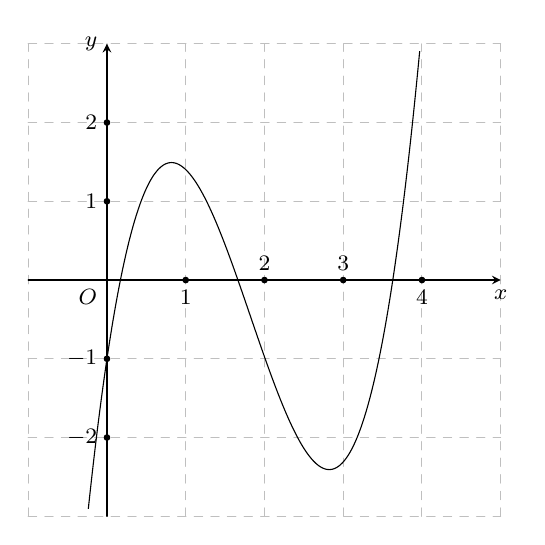
\begin{tikzpicture}[scale=1,>=stealth, font=\footnotesize, line join=round, line cap=round]
			\def\a{0.97} \def\b{-5.3} \def\c{6.733} \def\d{-1} % Hệ số
			\def\xmin{-1} \def\xmax{5}
			\def\ymin{-3} \def\ymax{3} 
			\draw[color=gray!50,dashed] (\xmin,\ymin) grid (\xmax,\ymax); 
			\draw[->] (\xmin,0)--(\xmax,0) node [below]{$x$};
			\draw[->] (0,\ymin)--(0,\ymax) node [left]{$y$};
			\node at (0,0) [below left]{$O$};
			\clip (\xmin+0.1,\ymin+0.1) rectangle (\xmax-0.5,\ymax-0.1);
			\draw[smooth,samples=300] plot(\x,{\a*(\x)^3+\b*(\x)^2+\c*(\x)+\d});
			\draw[fill=black] (2,0) node[above]{$2$} circle(1pt) (3,0)node[above]{$3$} circle(1pt) (4,0) node[below]{$4$}circle(1pt) (1,0) node[below]{$1$}circle(1pt) (0,-2) node[left]{$-2$}circle(1pt) (0,-1) node[left]{$-1$}circle(1pt) (0,1) node[left]{$1$}circle(1pt) (0,2) node[left]{$2$}circle(1pt);	
	\end{tikzpicture}}	
	\loigiai{Ta có số nghiệm phương trình $f(x)=m$ chính là số giao điểm của đồ thị $y=f(x)$ với đường thẳng $y=m$.\\
		Từ đồ thị trên, ta thấy để 	phương trình $f(x)=m$ có đúng $3$ nghiệm dương phân biệt thì $m=1$.			
	}
\end{ex}
\begin{ex}%[Thi thử tốt nghiệp - Liên trường THPT Nghệ An - 23]%[Huỳnh Xuân Tín - EX6]%[2D4K2-4]
	Trong mặt phẳng toạ độ, biết tập hợp các điểm biểu diễn của số phức $z$ thoả mãn $|z-i|=\sqrt{2}|z|$ là một đường tròn, tính bán kính đường tròn đó.	
	\choice
	{$2$}
	{$1$}
	{$\sqrt{3}$}
	{\True $\sqrt{2}$}
	\loigiai{
		Gọi $z=x+yi$ với $x, y\in \mathbb{R}$. Ta có
		\begin{eqnarray*}
			& & |z-i|=\sqrt{2}|z|\Leftrightarrow|x+yi-i|=\sqrt{2}|x+yi|\\
			&\Leftrightarrow & x^2+(y-1)^2=2x^2+y^2\Leftrightarrow x^2+y^2+2y-1=0\\
			&\Leftrightarrow & x^2+(y+1)^2=2.
		\end{eqnarray*}
		Vậy tập hợp các điểm biểu diễn của số phức $z$ thoả mãn $|z-i|=\sqrt{2}|z|$ là một đường tròn tâm $I(0;-1)$ bán kính $R=\sqrt{2}$.	
	}
\end{ex}
\begin{ex}%[Thi thử tốt nghiệp - Liên trường THPT Nghệ An - 23]%[Huỳnh Xuân Tín - EX6]%[1H3K5-3]
	\immini{Cho hình lăng trụ đứng $ABC.A'B'C'$ có chiều cao bằng $a \sqrt{3}$, có đáy $ABC$ là tam giác vuông tại $A$ và $AB=a$, $AC=2a$ (tham khảo hình vẽ). Khoảng cách từ $B$ đến mặt phẳng $\left(AB'C'\right)$ bằng
		\choice
		{$\dfrac{\sqrt{57}}{19} a$}
		{$\dfrac{3\sqrt{57}}{19} a$}
		{$\dfrac{\sqrt{57}}{38} a$}
		{\True $\dfrac{2\sqrt{57}}{19} a$}}{
		\begin{tikzpicture}[scale=0.7,>=stealth, font=\footnotesize, line join=round, line cap=round]
			\tkzDefPoints{0/0/A,1.1/-1.5/B,3.5/0/C}
			\coordinate (A') at ($(A)+(0,3.2)$);
			\tkzDefPointsBy[translation=from A to A'](B,C){B'}{C'}
			\tkzDrawPolygon(A,B,C,C',B',A')
			\tkzDrawSegments(A',C' B',B B',A)
			\tkzDrawSegments[dashed](A,C C',A)
			\tkzDrawPoints[fill=black](A,C,B,A',B',C')
			\tkzLabelPoints[above](B')
			\tkzLabelPoints[below](B)
			\tkzLabelPoints[left](A',A)
			\tkzLabelPoints[right](C',C)
	\end{tikzpicture}}	
	\loigiai{
		\immini{ Kẻ $A'H\perp B'C'$ (trong $(A'B'C')$). Suy ra $B'C'\perp (A'A'H)$\\
			Gọi $I$ là hình chiếu vuông góc của $A'$ lên $AH$.\\ Suy ra $AI\perp(AB'C')$ hay $AI=\mathrm{d}(A',(AB'C'))$.\\
			Ta có $A'B$ cắt mặt phẳng $(AB'C')$ tại trung điểm của $A'B$ nên\\ $\mathrm{d}(B,(AB'C'))=\mathrm{d}(A',(AB'C'))=AI$.\\
			Ta có $\dfrac{1}{A'H^2}=\dfrac{1}{A'B'^2}+\dfrac{1}{A'C'^2}=\dfrac{1}{a^2}+\dfrac{1}{4a^2}=\dfrac{5}{4a^2}\Rightarrow A'H=\dfrac{2\sqrt{5}a}{2}$.\\
			Ta có $\dfrac{1}{AI^2}=\dfrac{1}{A'A^2}+\dfrac{1}{A'H^2}=\dfrac{1}{3a^2}+\dfrac{5}{4a^2}=\dfrac{19}{12a^2}\Rightarrow A'I=\dfrac{2\sqrt{57}}{19} a$.\\
			Vậy khoảng cách từ $B$ đến mặt phẳng $\left(AB'C'\right)$ bằng $\dfrac{2\sqrt{57}}{19} a$. }{
			\begin{tikzpicture}[scale=0.7,>=stealth, font=\footnotesize, line join=round, line cap=round]
				\tkzDefPoints{0/0/A,1.5/-1.5/B,4.5/0/C}
				\coordinate (A') at ($(A)+(0,4.5)$);
				\tkzDefPointsBy[translation=from A to A'](B,C){B'}{C'}
				\coordinate (H) at ($(B')!0.4!(C')$);
				\coordinate (I) at ($(A)!0.6!(H)$);
				\tkzDrawPolygon(A,B,C,C',B',A')
				\tkzDrawSegments(A',C' B',B B',A A',B A',H)
				\tkzDrawSegments[dashed](A,C C',A A,H A',I)
				\tkzDrawPoints[fill=black](A,C,B,A',B',C',H,I)
				\tkzLabelPoints[above](B',H)
				\tkzLabelPoints[below](B,I)
				\tkzLabelPoints[left](A',A)
				\tkzLabelPoints[right](C',C)
		\end{tikzpicture}}		
	}
\end{ex}
\begin{ex}%[Thi thử tốt nghiệp - Liên trường THPT Nghệ An - 23]%[Huỳnh Xuân Tín - EX6]%[1D2K5-2]
	Một hộp đựng $13$ quả cầu gồm: $7$ quả cầu màu vàng đánh số từ $1$ đến $7$, $6$ quả cầu màu đỏ đánh số từ $1$ đến $6$. Lấy ngẫu nhiên hai quả, tính xác suất để hai quả đó khác màu và khác số.	
	\choice
	{$\dfrac{5}{13}$}
	{$\dfrac{7}{13}$}
	{$\dfrac{35}{78}$}
	{\True $\dfrac{6}{13}$}
	\loigiai{
		Số cách chọn $2$ quả từ hộp trên là $|\Omega|=\mathrm{C}_{13}^2=78$.\\
		Gọi $A$ là \,\lq\lq biến cố nhận được hai quả cầu khác màu và khác số\rq\rq.
		\begin{itemize}
			\item Số cách chọn một quả cầu đỏ là $6$.
			\item Số cách chọn một quả cầu vàng là $6$ (trừ một quả cầu vàng có cùng số với quả cầu đỏ vừa chọn).
		\end{itemize}		
		Suy ra $|A|=6\cdot 6=36$.\\
		Vậy xác suất để hai quả đó khác màu và khác số là $\mathrm{P}(A)=\dfrac{|A|}{|\Omega|}=\dfrac{36}{78}=\dfrac{6}{13}$.
	}
\end{ex}
\begin{ex}%[Thi thử tốt nghiệp - Liên trường THPT Nghệ An - 23]%[Huỳnh Xuân Tín - EX6]%[1H3K4-3]
	\immini{ Cho hình chóp $S.A B C$ có đáy là tam giác vuông cân tại $A$, $S A$ vuông góc với đáy và $S A=\sqrt{\dfrac{3}{2}} \cdot A B$. Góc giữa hai mặt phẳng $(S B C)$ và $(A B C)$ bằng 	\choice
		{$45^\circ$}
		{\True$60^\circ$}
		{$30^\circ$}
		{ $\arctan\sqrt{\dfrac{3}{2}}$}}{
		\begin{tikzpicture}[scale=0.7,>=stealth, font=\footnotesize, line join=round, line cap=round]
			\tkzDefPoints{0/0/A,1.2/-1.5/B,4/0/C}
			\coordinate (S) at ($(A)+(0,3)$);
			\tkzDrawPolygon(S,A,B,C)
			\tkzDrawSegments(S,B)
			\tkzDrawSegments[dashed](A,C)
			\tkzDrawPoints[fill=black](A,B,C,S)
			\tkzMarkRightAngles[size=0.16](S,A,B S,A,C)
			\tkzLabelPoints[above](S)
			\tkzLabelPoints[below](B)
			\tkzLabelPoints[left](A)
			\tkzLabelPoints[right](C)
	\end{tikzpicture}}	
	\loigiai{
		\immini{ Gọi $I$ là trung điểm $BC$.\\
			Vì $\triangle ABC$ vuông cân tại $A$ nên $AI\perp BC$.\\
			Suy ra $SI\perp BC$. Mặt khác $(SBC)\cap (ABC)=BC$ suy ra góc giữa hai mặt phẳng $(S B C)$ và $(A B C)$ bằng $\widehat{SIA}$.\\
			Ta có $AI=\dfrac{AB}{\sqrt{2}}$ (vì $\triangle AIB$ vuông cân).\\
			Ta có $\tan\widehat{SIA}=\dfrac{SA}{AI}=\dfrac{SA\sqrt{2}}{AB}=\dfrac{\sqrt{2}}{1}\cdot \sqrt{\dfrac{3}{2}}=\sqrt{3}$.\\
			Vậy góc giữa hai mặt phẳng $(S B C)$ và $(A B C)$ bằng $60^\circ$.}{
			\begin{tikzpicture}[scale=0.7,>=stealth, font=\footnotesize, line join=round, line cap=round]
				\tkzDefPoints{0/0/A,1.2/-1.5/B,4/0/C}
				\coordinate (S) at ($(A)+(0,3)$);
				\coordinate ({I}) at ($(C)!0.5!(B)$);	
				\tkzDrawPolygon(S,A,B,C)
				\tkzDrawSegments(S,B S,I)
				\tkzDrawSegments[dashed](A,C A,I)
				\tkzDrawPoints[fill=black](A,B,C,S,I)
				\tkzMarkRightAngles[size=0.16](S,A,B S,A,C)
				\tkzLabelPoints[above](S)
				\tkzLabelPoints[below](B,I)
				\tkzLabelPoints[left](A)
				\tkzLabelPoints[right](C)
		\end{tikzpicture}}			
	}
\end{ex}
\begin{ex}%[Thi thử tốt nghiệp - Liên trường THPT Nghệ An - 23]%[Huỳnh Xuân Tín - EX6]%[2D4K4-2]
	Trên tập hợp số phức, cho phương trình $z^2+a z+b=0$ (với $a, b$ là số thực). Biết rằng hai số phức $w+1+i$ và $2 w-1+5 i$ là hai nghiệm của phương trình đã cho. Tính tổng $a+b$.	
	\choice
	{$9$}
	{$16$}
	{$1$}
	{\True $4$}
	\loigiai{Ta có $z^2+a z+b=0$ (với $a, b$ là số thực).\hfill{(1)}
		\begin{enumerate}[TH 1.]
			\item (1) có hai nghiệm không phải là nghiệm thực. Giả sử $w=x+yi$ với $x,y\in \mathbb{R}$.\\
			Khi đó $z_1=w+1+i=x+1+(y+1)i$ và $z_2=2w-1+5i=2x-1+(2y+5)i$.\\
			Vì $z_1$ và $z_2$ là hai nghiệm phức của (1) nên $z_1=\overline{z}_2$.
			\[x+1+(y+1)i=2x-1-(2y+5)i\Leftrightarrow \heva{&x+1=2x-1\\&y+1=-2y-5}\Leftrightarrow\heva{&x=2\\&y=-2}\Rightarrow\heva{&z_1=3-i\\&z_2=3+i.}\]
			Suy ra $\heva{&z_1+z_2=-a=3-i+3+i=6\\&z_1z_2=b=10}\Rightarrow \heva{&a=-6\\&b=10.}$\\
			Suy ra $a+b=4$.
			\item (1) có hai nghiệm thực. Giả sử $w=x+yi$ với $x,y\in \mathbb{R}$.\\
			Khi đó $z_1=w+1+i=x+1+(y+1)i$ và $z_2=2w-1+5i=2x-1+(2y+5)i$ là số thực.\\
			Suy ra $\heva{&y+1=0\\&2y+5=0}\Leftrightarrow\heva{&y=-1\\&y=-\dfrac{5}{2}}$ vô nghiệm. Do đó trường hợp này không xảy ra.
		\end{enumerate}		
	}
\end{ex}
\begin{ex}%[Thi thử tốt nghiệp - Liên trường THPT Nghệ An - 23]%[Huỳnh Xuân Tín - EX6]%[2D2K6-3]
	Có bao nhiêu giá trị nguyên thuộc $[-20 ; 20]$ của tham số $m$ để bất phương trình $4^x-(m+1) 2^x+m \leq 0$ có tập nghiệm là một đoạn có độ dài lớn hơn $2$?	
	\choice
	{$17$}
	{$37$}
	{$38$}
	{\True $16$}
	\loigiai{
		Đặt $t=2^x$, điều kiện $t>0$. Khi đó bất phương trình	$4^x-(m+1) 2^x+m \leq 0$ được viết lại
		\[t^2-(m+1)t+m\le0.\qquad (*)\]
		Do đó để để bất phương trình $4^x-(m+1) 2^x+m \leq 0$ có tập nghiệm là một đoạn $[x_1;x_2]$, có độ dài lớn hơn $2$ tức là $\left|x_1-x_2\right|>2$  thì bất phương trình (*) có tập nghiệm dạng $\left[t_1;t_2\right]$ với $0<t_1<t_2$ và $\left|\log_2t_2-\log_2t_1\right|>2$ với $t_1$, $t_2$ là hai nghiệm của phương trình $t^2-(m+1)t+m=0$ (có $\Delta=(m+1)^2-4m=(m-1)^2$).\hfill{(**)}\\
		Suy ra $\hoac{&t_1=\dfrac{m+1+m-1}{2}=m\\&t_2=\dfrac{m+1-m+1}{2}=1.}$\\
		Khi đó điều kiện (**) tương đương với 
		\[\heva{&m>0\\&\left|\log_2m-\log_21\right|>2}\Leftrightarrow\heva{&m>0\\&\log_2m>2}\Leftrightarrow m>4.\]
		Vì $m$ nguyên thuộc $[-20;20]$ nên $m\in \{5;6\cdots;19;20\}$.\\Vậy số giá trị nguyên $m$ thỏa bài toán là $16$.
	}
\end{ex}
\begin{ex}%[Thi thử tốt nghiệp - Liên trường THPT Nghệ An - 23]%[Huỳnh Xuân Tín - EX6]%[2H2K1-4]
	\immini{Người ta sản xuất thùng phuy sắt có hình dạng là một hình trụ (có nắp đậy kín) bằng cách cán và gò các tấm thép có độ dày $1 \mathrm{~mm}$, biết chiều cao của thùng phuy là $876 \mathrm{~mm}$, đường kính ngoài của thùng phuy là $580 \mathrm{~mm}$ và khối lượng riêng của thép là $7850 \mathrm{~kg} / \mathrm{m}^3$. Hỏi mỗi thùng phuy nặng khoảng bao nhiêu $\mathrm{kg}$ (tính gần đúng sau dấu phẩy đến 2 chữ số thập phân)? \choice
		{$15{,}57$ kg}
		{$18{,}23$ kg}
		{\True $16{,}63$ kg}
		{$17{,}21$ kg}}{
		\begin{tikzpicture}[scale=0.8,>=stealth, font=\footnotesize, line join=round, line cap=round]
			\def \x{1.8} %bán kính trục lớn elip
			\def \y{0.8} %bán kính trục bé elip
			\def \h{3.5} %chiều cao hình trụ
			\coordinate (A) at (0,0);
			\coordinate (B) at (2*\x,0);
			\coordinate (O) at ($(A)!0.5!(B)$);
			\coordinate (O') at ($(O)+(0,\h)$);
			\coordinate (A') at ($(A)+(0,\h)$);
			\coordinate (B') at ($(B)+(0,\h)$);
			%Lấy các điểm M,N trên elip
			\coordinate (M) at ($(O)+({\x*cos(70)},{\y*sin(70)})$);
			\coordinate (N) at ($(O)+({\x*cos(-40)},{\y*sin(-40)})$);
			\coordinate (P) at ($(N)+(0,\h)$);
			\coordinate (Q) at ($(M)+(0,\h)$);
			\draw[dashed] (B) arc(0:180:\x cm and \y cm);
			\draw (B) arc(0:-180:\x cm and \y cm);
			\draw (O') ellipse (\x cm and \y cm);
			\tkzDrawSegments(A,A' B,B')
	\end{tikzpicture}}		
	\loigiai{
		\immini{Bán kính ngoài của thùng phuy là $R_1=\dfrac{580}{2}=290$ mm $=0{,}29$ m.	\\	
			Chiều cao bên ngoài thùng phuy là $h_1=0{,}876$. Khi đó có thể tích là
			\[V_1=\pi \cdot h_1\cdot R_1^2=\pi \cdot 0{,}876\cdot 0{,}29=0{,}0736716\pi.\]
			Bán kính trong của thùng phuy là $R_2=\dfrac{580-2}{2}=289$ mm $=0{,}289$ m.		\\
			Chiều cao bên trong thùng phuy là $h_2=0{,876}-0{,}002=0{,}874$. Khi đó thể tích bên trong thùng phuy là
			\[V_2=\pi \cdot h_2\cdot R_2^2=\pi \cdot 0{,}874\cdot 0{,}289^2=0{,}072997354\pi.\]
			Thể tích sắt cần làm thành thùng phuy \[V_1-V_2=0{,}0736716\pi-0{,}072997354\pi=6.74246\pi\cdot10^{-4} \left( \text{m}^3\right) .\]}{
			\begin{tikzpicture}[scale=0.5,>=stealth, font=\footnotesize, line join=round, line cap=round]
				\def\x{5} %bán trục lớn
				\def\y{1.3} %bán trục bé
				\def\h{9} %chiều cao trụ
				\def\a{4} %bán trục lớn
				\def\b{1.04} %bán trục bé
				\coordinate (B) at (0,0);
				\coordinate (A) at (-2*\x,0);
				\coordinate (O) at ($(A)!0.5!(B)$);
				\coordinate (O') at ($(O)+(0,\h)$);
				\coordinate (M') at ($(O')+(\a,0)$);
				\coordinate (N') at ($(O')-(\a,0)$);
				\coordinate (I) at ($(O)+(0,1)$);
				\coordinate (M) at ($(I)+(\a,0)$);
				\coordinate (N) at ($(I)-(\a,0)$);
				\coordinate (I) at ($(O)+(0,1)$);
				\coordinate (A') at ($(A)+(0,\h)$);
				\coordinate (B') at ($(B)+(0,\h)$);
				\draw[dashed] (B) arc (0:180:\x cm and \y cm);
				\draw[line width=0.5pt] (B) arc (0:-180:\x cm and \y cm);
				\draw (O') ellipse (\x cm and \y cm);
				\draw (O') ellipse (\a cm and \b cm);
				\draw[dashed] (I) ellipse (\a cm and \b cm);
				\tkzDrawSegments[thick](A',A B',B)
				\tkzDrawSegments[dashed](N,N' M',M)
		\end{tikzpicture}}
		\noindent Khối lượng mỗi thùng phuy là 
		\[\left(6{,}74246\pi\cdot10^{-4}\right)  \cdot7850\approx16{,}63 \text{kg}.\]		
	}
\end{ex}
\begin{ex}%[Thi thử tốt nghiệp - Liên trường THPT Nghệ An - 23]%[Huỳnh Xuân Tín - EX6]%[2H1K3-2]
	Cho hình lăng trụ đều $A B C.A' B' C'$ có cạnh đáy bằng $a$. Hai đường thẳng $A B'$ và $B C'$ vuông góc với nhau. Tính thể tích của khối lăng trụ đó.	
	\choice
	{$\dfrac{a^3 \sqrt{3}}{24}$}
	{\True $\dfrac{a^3 \sqrt{6}}{8}$}
	{$\dfrac{a^3 \sqrt{6}}{24}$}
	{$\dfrac{a^3 \sqrt{3}}{8}$}
	\loigiai{
		\immini{Đặt $AA'=x$. Gọi $H$ là trung điểm của $A'B'$. Suy ra $C'H\perp A'B'$.\\
			Vì $A'A\perp (A'B'C')$ nên $C'H\perp (ABB'A')$. Do đó $C'H\perp AB'$.\\
			Từ $\heva{&AB'\perp C'H\\&AB'\perp BC'}\Rightarrow AB'\perp (BC'H)\Rightarrow AB'\perp BH$ tại $I$.\\
			Ta có $AB\parallel B'H\Rightarrow \dfrac{ AI}{IB'}=\dfrac{BI}{IH}=\dfrac{AB}{B'H}=2\Rightarrow AI=\dfrac{2AB'}{3}=\dfrac{2\sqrt{x^2+a^2}}{3}$.\\
			$BI=\dfrac{2BH}{3}=\dfrac{2}{3}\sqrt{x^2+\dfrac{a^2}{4}}$.\\
			Ta có $\triangle AIB$  vuông tại $I$ nên $AB^2=AI^2+BI^2$\\
			$\Leftrightarrow a^2=\dfrac{4}{9}(x^2+a^2)+\dfrac{4}{9}\left(x^2+\dfrac{a^2}{4}\right)\Leftrightarrow x^2=\dfrac{a^2}{2}\Leftrightarrow x=\dfrac{a\sqrt{2}}{2}$ hay $AA'=\dfrac{a\sqrt{2}}{2}$. }{
			\begin{tikzpicture}[scale=1,>=stealth, font=\footnotesize, line join=round, line cap=round]
				\tkzDefPoints{0/0/A,1.1/-1.5/B,3.5/0/C}
				\coordinate (A') at ($(A)+(0,3.2)$);
				\tkzDefPointsBy[translation=from A to A'](B,C){B'}{C'}
				\tkzDrawPolygon(A,B,C,C',B',A')
				\coordinate (H) at ($(A')!0.5!(B')$);
				\tkzInterLL(A,B')(B,H)\tkzGetPoint{I}
				\tkzDrawSegments(A',C' B',B A,B' B,C' A,B' B,H)
				\tkzDrawSegments[dashed](A,C C',H)
				\tkzDrawPoints[fill=black](A,C,B,A',B',C',I,H)
				\tkzLabelPoints[above](B')
				\tkzLabelPoints[below](B)
				\tkzLabelPoints[left](A',A,I,H)
				\tkzLabelPoints[right](C',C)
		\end{tikzpicture}}		
		\noindent Vậy thể tích lăng trụ là 	$V=AA'\cdot S_{ABC}=\dfrac{a \sqrt{2}}{2} \cdot \dfrac{a^2 \sqrt{3}}{4}=\dfrac{a^3 \sqrt{6}}{8}$.	
	}
\end{ex}
\begin{ex}%[Thi thử tốt nghiệp - Liên trường THPT Nghệ An - 23]%[Huỳnh Xuân Tín - EX6]%[2D1K2-6]
	Cho hàm số $f(x)=\dfrac{1}{3} x^3-(m-1) x^2+\left(m^2-16\right) x+2023$. Có bao nhiêu giá trị nguyên của tham số $m$ để hàm số $g(x)=f(|x|)$ có $5$ điểm cực trị?	
	\choice
	{\True $4$}
	{$5$}
	{Vô số}
	{$3$}
	\loigiai{Ta có $f'(x)=x^2-2(m-1)x+m^2-16$.\\
		Hàm số $f(|x|)$ có $5$ điểm cực trị khi $f(x)$ có $2$ điểm cực trị dương.\\
		Hay $f'(x)=0$ có hai nghiệm dương
		\[\heva{&\Delta'>0\\&-\dfrac{b}{a}>0\\&\dfrac{c}{a}>0}\Leftrightarrow\heva{&(m-1)^2-m^2+16>0\\&m-1>0\\&m^2-16>0}\Leftrightarrow \heva{&-2m+17>0\\&m>1\\&m<-4,\, m>4}\Leftrightarrow 4<m<\dfrac{17}{2}.\]	
		Vì $m\in \mathbb{Z}$ nên $m\in \{5;6;7;8\}$.\\
		Vậy có $4$ giá trị nguyên của $m$ thỏa bài toán.	
	}
\end{ex}
\begin{ex}%[Thi thử tốt nghiệp - Liên trường THPT Nghệ An - 23]%[Huỳnh Xuân Tín - EX6]%[2D3G3-3]
	\immini{Cho hàm số $y=f(x)$ có đạo hàm cấp hai liên tục trên $\mathbb{R}$, biết rằng $f(0)=0$ và hàm số $g(x)=\dfrac{1}{16}\left[x f''(x)+f'(x)\right]$ là hàm số bậc ba có đồ thị như hình vẽ. Thể tích khối tròn xoay sinh bởi hình phẳng giới hạn bởi các đồ thị hàm số $y=f(x)$, $y=\dfrac{f^{\prime \prime}(x)-40}{12}$ khi quay quanh trục $O x$ có giá trị nằm trong khoảng nào sau đây? 	\choice
		{$(116;117)$}
		{\True $(117;118)$}
		{$(118;119)$}
		{$(115;116)$}}{
		\begin{tikzpicture}[scale=0.6,>=stealth, font=\footnotesize, line join=round, line cap=round]
			\def\a{1} \def\b{0} \def\c{-1} \def\d{0} % Hệ số
			\def\xmin{-2} \def\xmax{3}
			\def\ymin{-2} \def\ymax{7} 
			\draw[->] (\xmin,0)--(\xmax,0) node [below]{$x$};
			\draw[->] (0,\ymin)--(0,\ymax) node [left]{$y$};
			\node at (0,0) [below left]{$O$};
			\clip (\xmin+0.1,\ymin+0.1) rectangle (\xmax-0.5,\ymax-0.1);
			\draw[smooth,samples=300] plot(\x,{\a*(\x)^3+\b*(\x)^2+\c*(\x)+\d});
			\draw[fill=black] (2,0) node[below]{$2$} circle(1pt)  (1,0) node[below right]{$1$}circle(1pt) (-1,0) node[above left]{$-1$}circle(1pt)  (0,6) node[left]{$6$}circle(1pt);	
			\draw[dashed](2,0)--(2,6)--(0,6);		
	\end{tikzpicture}}	
	\loigiai{
		Nhìn vào đồ thị ta thấy $y=g(x)$ là hàm số bậc ba, cắt trục hoành tại $3$ điểm và đi qua điểm $(2;6)$ nên
		\[\heva{&g(x)=ax(x+1)(x-1)\\&g(2)=6}\Leftrightarrow a=1\Leftrightarrow g(x)=x^3-x.\]
		Ta có $g(x)=\dfrac{1}{16}\left[x f''(x)+f'(x)\right]=\dfrac{1}{16}[x\cdot f'(x)]'=x^3-x\Rightarrow x\cdot f'(x)=4x^4-8x^2+C$.\\
		Ta có $g(0)=0\Rightarrow f'(0)=0\Rightarrow C=0\Rightarrow f'(x)=4x^3-8x$.	\\
		Khi đó $f(x)=x^4-4x^2+C_1$. Vì $f(0)=0\Rightarrow C_1=0$.\\
		Do đó $f(x)=x^4-4x^2$ và $f'(x)=4x^3-8x\Rightarrow f''=(x)=12x^2-8$.\\
		Hàm số $y=h(x)=\dfrac{f''(x)-40}{12}=x^2-4$.\\
		Phương trình hoành độ giao điểm của $y=f(x)$ và $y=h(x)$ là
		\[x^4-4x^2=x^2-4\Leftrightarrow x^4-3x^2+4=0\Leftrightarrow \hoac{&x=\pm2\\&x=\pm 1.}\]
		Khi đó thể tích khối tròn xoay sinh bởi hình phẳng giới hạn bởi các đồ thị hàm số $y=f(x)$, $y=h(x)$ khi quay quanh trục $O x$ là 
		\[V=\pi \displaystyle\int\limits_{-2}^2 \left|f^2(x)-h^2(x)\right|\mathrm{\,d}x=\pi \displaystyle\int\limits_{-2}^2 \left|f^2(x)-g^2(x)\right|\mathrm{\,d}x=\pi \displaystyle\int\limits_{-2}^2 \left|x^8-8x^6+15x^4+8x^2-16\right|\mathrm{\,d}x\]
		$= \left|\displaystyle\int\limits_{-2}^{-1} \left(x^8-8x^6+15x^4+8x^2-16\right)\mathrm{\,d}x \right|+\pi\left|\displaystyle\int\limits_{-1}^{1} \left(x^8-8x^6+15x^4+8x^2-16\right)\mathrm{\,d}x \right|+\pi\left|\displaystyle\int\limits_{1}^{2} \left(x^8-8x^6+15x^4+8x^2-16\right) \mathrm{\,d}x \right| \\
		=\pi \left|\displaystyle\int\limits_{-2}^{-1} \left(x^8-8x^6+15x^4+8x^2-16\right)\mathrm{\,d}x \right|+\pi\left|\displaystyle\int\limits_{-1}^{1} \left(x^8-8x^6+15x^4+8x^2-16\right)\mathrm{\,d}x \right|+\pi\left|\displaystyle\int\limits_{1}^{2} \left(x^8-8x^6+15x^4+8x^2-16\right)\mathrm{\,d}x \right| \\
		=\dfrac{460\pi}{63}+\dfrac{1432\pi}{63}+\dfrac{460\pi}{63}=\dfrac{112\pi}{3}\approx 117{,}28.$\\
		Vậy thể tích cần tìm là $V\in (117;118)$.	
	}
\end{ex}
\begin{ex}%[Thi thử tốt nghiệp - Liên trường THPT Nghệ An - 23]%[Huỳnh Xuân Tín - EX6]%[2H3G3-8]
	Trong không gian với hệ trục toạ độ $O x y z$, cho hai điểm $A(3 ; 1 ; 2)$, $B(1 ;-1 ; 2)$ và mặt phẳng $(P)\colon x+y+2 z-18=0$. Khi điểm $M$ thay đổi trên mặt phẳng $(P)$ lấy điểm $N$ thuộc tia $O M$ sao cho $O M \cdot O N=36$. Tìm giá trị nhỏ nhất của biểu thức $N A^2+N B^2$.	
	\choice
	{$16-8 \sqrt{3}$}
	{$24-8 \sqrt{3}$}
	{\True $20-8 \sqrt{3}$}
	{$8-4 \sqrt{3}$}
	\loigiai{
		\immini{Gọi $H$ là hình chiếu vuông góc của $O$ lên $(P)$. Suy ra đường thẳng $OH$ là $\heva{&x=t\\&y=t\\&z=2t.}$\\
			Khi đó tọa độ điểm $H$ là nghiệm hệ phương trình
			\[\heva{&x=t\\&y=t\\&z=2t\\&x+y+2z-18=0}\Leftrightarrow \heva{&x=3\\&y=3\\&z=6}
			\Rightarrow H(3;3;6),\quad OH=3\sqrt{6}.\]
		}{
			\begin{tikzpicture}[scale=0.8,>=stealth, font=\footnotesize, line join=round, line cap=round]
				\tkzDefPoints{0/0/E,5/0/F,7/3/G,2/3/D,3/1/H,3/5/O,4/0.6/M}
				\coordinate (N) at ($(O)!0.4!(M)$);
				\coordinate (K) at ($(O)!0.7!(H)$);
				\coordinate (J) at ($(O)!0.5!(K)$);
				\tkzDrawSegments(O,M O,H H,M N,K E,F F,G G,D D,E)
				\tkzDrawPoints[fill=black](H,M,N,K,J,O)
				\foreach \p/\r in {H/-180,J/-180,K/-180,O/-180,N/45,M/0}
				\fill (\p) circle (1.5pt) node[shift={(\r:3mm)}]{$\p$};		
		\end{tikzpicture}}		
		\noindent Trên tia $OH$ lấy điểm $K$ sao cho $OH\cdot OK=36\Rightarrow OK=2\sqrt{6}$.\\
		Suy ra $\overrightarrow{OK}=\dfrac{2}{3}\overrightarrow{OH}\Rightarrow K(2;2;4)$.\\
		Ta có $OH\cdot OK=OM\cdot ON\Rightarrow \dfrac{OH}{ON}=\dfrac{OM}{OK}\Rightarrow \triangle OHM\simeq \triangle ONK$.\\
		$\Rightarrow \widehat{ONK}=\widehat{OHM}=90^\circ$. Khi đó $N$ thuộc mặt cầu tâm $J(1;1;2)$ (trung điểm của $OK$) bán kính $R=\dfrac{OK}{2}=\sqrt{6}$.		\\
		Gọi $I$ là trung điểm $AB$. Suy ra $I(2;0;2)$.\\
		Xét $\triangle NAB$ với trung tuyến $NI$. Ta có
		$$N A^2+N B^2=2NI^2+\dfrac{AB^2}{2}=2NI^2+4.$$
		Vì $N$ thuộc mặt cầu tâm $J(1;1;2)$ bán kính $R=\sqrt{6}$ nên $NI\ge |IJ-R|=\sqrt{6}-\sqrt{2}$.\\
		Khi đó $NA^2+NB^2\ge 2\left(\sqrt{6}-\sqrt{2}\right)^2+4=20-8\sqrt{3}$.\\
		Vậy giá trị nhỏ nhất của biểu thức $N A^2+N B^2$ là $20-8\sqrt{3}$.	}
\end{ex}
\begin{ex}%[Thi thử tốt nghiệp - Liên trường THPT Nghệ An - 23]%[Huỳnh Xuân Tín - EX6]%[2D1G5-5]
	Cho hàm số $y=f(x)$ có đạo hàm là $f'(x)=(x-a)(x-b)$ với $a$, $b$ là hai hằng số và $a<b$, biết rằng $f(b)=0$ và hàm số $g(x)=\left|4 x^3+(2-3 f(a)) x^2-2 f(a) x+m\right|$ (với $m$ là tham số). Khi đó hàm số $g[f(x)]$ có tối đa bao nhiêu điểm cực trị?	
	\choice
	{$17$}
	{$11$}
	{\True $13$}
	{$15$}
	\loigiai{
		\immini{Từ $f'(x)=(x-a)(x-b)$ với $a$, $b$ là hai hằng số và $a<b$, $f(b)=0$ ta suy ra đồ thị $y=f(x)$ có dạng như hình bên.\\
			Đặt $h(x)=4 x^3+(2-3 f(a)) x^2-2 f(a) x+m$.\\
			Ta có $h'(x)=12x^2+2(2-3f(a))x-2f(a)$. Xét $h'(x)=0\Leftrightarrow\hoac{&x=-\dfrac{1}{3}\\&x=\dfrac{f(a)}{2}>0.}$\\
			Ta có $g(x)=|h(x)|=\sqrt{h^2(x)}\Rightarrow g'(x)=\dfrac{h'(x)\cdot h(x)}{|h(x)|}$.\\
			Xét $g'(x)=0\Leftrightarrow \hoac{&h'(x)=0\Leftrightarrow x\in \left\lbrace -\dfrac{1}{3};\dfrac{f(a)}{2} \right\rbrace \\
				&h(x)=0.}$}{
			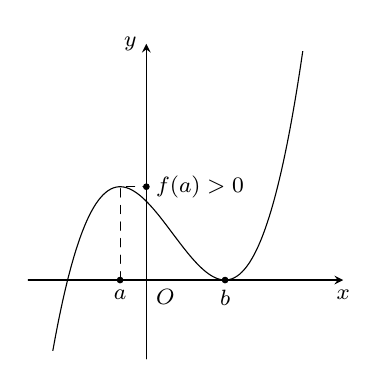
\begin{tikzpicture}[scale=1,>=stealth, font=\footnotesize, line join=round, line cap=round]
				\def\a{1} \def\b{-1} \def\c{-1} \def\d{1} % Hệ số
				\def\xmin{-1.5} \def\xmax{2.5}
				\def\ymin{-1} \def\ymax{3} 
				%	\draw[color=gray!50,dashed] (\xmin,\ymin) grid (\xmax,\ymax); 
				\draw[->] (\xmin,0)--(\xmax,0) node [below]{$x$};
				\draw[->] (0,\ymin)--(0,\ymax) node [left]{$y$};
				\node at (0,0) [below right]{$O$};
				\clip (\xmin+0.1,\ymin+0.1) rectangle (\xmax-0.5,\ymax-0.1);
				\draw[smooth,samples=300] plot(\x,{\a*(\x)^3+\b*(\x)^2+\c*(\x)+\d});
				\draw[fill=black] (1,0) node[below]{$b$} circle(1pt) (-1/3,0)node[below]{$a$} circle(1pt)  (0,32/27) node[right]{$f(a)>0$}circle(1pt);	
				\draw[dashed] (-1/3,0)--(-1/3,32/27)--(0,32/27);	
		\end{tikzpicture}}		
		\noindent Ta có bảng biến thiên của $h(x)$ như sau
		\begin{center}
			
\begin{tikzpicture}
				\tkzTabInit[nocadre=false,lgt=1.2,espcl=2.5,deltacl=0.6]
				{$x$ /1.2, $h'(x)$ /0.6, $h(x)$ /2.5}
				{$-\infty$,$-\dfrac{1}{3}$,$\dfrac{f(a)}{2}$,$+\infty$}
				\tkzTabLine{,+,$0$,-,$0$,+,}
				\tkzTabVar{-/$-\infty$,+/,-/,+/$+\infty$}
			\end{tikzpicture}
		\end{center}	
		Từ bảng biến thiên trên ta thấy $h(x)=0$ có tối đa ba nghiệm  phân biệt $x_1$, $x_2$, $x_3$ thỏa $x_1<-\dfrac{1}{3}<x_2<\dfrac{f(a)}{2}<x_3$.\\
		Xét $y=g[f(x)]$. Ta có $y'=f'(x)\cdot g'[f(x)]$.\\
		Với $y'=0\Leftrightarrow \hoac{&f'(x)=0\\&g'[f(x)]=0}\Leftrightarrow\hoac{&x\in \{a;b\}\\&f(x)=-\dfrac{1}{3}\qquad(1)\\&f(x)=\dfrac{f(a)}{2}>0\qquad(2)\\&f(x)=x_1<-\dfrac{1}{3}\qquad(3)\\&f(x)=x_2\in \left(-\dfrac{1}{3};\dfrac{f(a)}{2}\right)\qquad(4)\\&f(x)=x_3>0. \qquad(5)}$	\\
		Nhìn vào đồ thị của hàm số $y=f(x)$ ta thấy
		\begin{itemize}
			\item Đường thẳng $y=-\dfrac{1}{3}$ cắt đồ thị $y=f(x)$ tại một điểm nên (1) có đúng một nghiệm đơn.
			\item Đường thẳng $y=\dfrac{f(a)}{2}$ cắt đồ thị $y=f(x)$ tối đa tại ba điểm phân biệt nên (2) có tối đa ba nghiệm phân biệt.
			\item Đường thẳng $y=x_1$ cắt đồ thị $y=f(x)$ tại một điểm nên (3) đúng có một nghiệm đơn.	
			\item Đường thẳng $y=x_2$ cắt đồ thị $y=f(x)$ tối đa tại ba điểm phân biệt nên (4) có tối đa ba nghiệm phân biệt.
			\item Đường thẳng $y=x_3$ cắt đồ thị $y=f(x)$ tối đa tại ba điểm phân biệt nên (5) có tối đa ba nghiệm phân biệt.
		\end{itemize}
		Vậy hàm số $y=g[f(x)]$ có tối đa $2+1+3+1+3+3=13$ cực trị.
	}
\end{ex}
\begin{ex}%[Thi thử tốt nghiệp - Liên trường THPT Nghệ An - 23]%[Huỳnh Xuân Tín - EX6]%[2H3G3-7]
	Trong không gian $O x y z$, cho mặt phẳng $(P)\colon 2 x+a y+b z+c=0$ chứa đường thẳng $d$ là giao tuyến của hai mặt phẳng $(\alpha)\colon x+y-z+1=0$, $(\beta)\colon x+y-2 z-1=0$. Biết rằng khoảng cách từ điểm $M(1 ; 2 ; 1)$ đến mặt phẳng $(P)$ bằng $3$. Khi đó giá trị $a+b+c$ bằng	
	\choice
	{$3$}
	{$4$}
	{\True $5$}
	{$6$}
	\loigiai{
		$(\alpha)\colon x+y-z+1=0$ có véc-tơ pháp tuyến là $\overrightarrow{n}_1=(1;1;-1)$; $(\beta)\colon x+y-2 z-1=0$ có véc-tơ pháp tuyến là $\overrightarrow{n}_2=(1;1;-2)$.\\
		Vì  $d$ là giao tuyến của hai mặt phẳng $(\alpha)$ và $(\beta)$ nên $d$ có véc-tơ chỉ phương là $\overrightarrow{v}=\left[\overrightarrow{n}_1,\overrightarrow{n}_2\right]=(-1;1-0)$ và $d$ đi qua điểm $A(0;y;z)$, với $y$; $z$ là nghiệm của $\heva{&y-z+1=0\\&y-2z-1=0}\Leftrightarrow \heva{&y=-3\\&z=-2}\Rightarrow A(0;-3;-2)$\\
		Khi đó phương trình của $d$ là $\heva{&x=-t\\&y=-3+t\\&z=-2.}$\\
		Vì mặt phẳng $(P)$ chứa $d$ nên
		\[\heva{&\overrightarrow{v}\cdot \overrightarrow{n}_P=0\\&A\in (P)}\Leftrightarrow \heva{&-2+a=0\\&-3a-2b+c=0}\Leftrightarrow \heva{&a=2\\&c=2b+6.}\]
		Suy ra $(P)\colon 2x+2y+bz+2b+6=0$.	\\
		Ta có khoảng cách từ điểm $M(1 ; 2 ; 1)$ đến mặt phẳng $(P)$ bằng $3$
		\[\dfrac{|2+4+b+2b+6|}{\sqrt{8+b^2}}=3\Leftrightarrow|b+4|=\sqrt{b^2+8}\Leftrightarrow b^2+8b+16=b^2+8\Leftrightarrow b=-1.\]
		Vậy $a=2$, $b=-1$, $c=4$. Khi đó $a+b+c=5$.
	}
\end{ex}
\begin{ex}%[Thi thử tốt nghiệp - Liên trường THPT Nghệ An - 23]%[Huỳnh Xuân Tín - EX6]%[2D4G5-1]
	Cho số phức $z$ thỏa mãn $\left| (1+i) z+(1-i) \bar{z}\right| +\left| (1+i) z-(1-i) \bar{z}\right| =4$ và số phức $u$ thỏa mãn $(u-1+3 i)(i\overline{u}-3+5 i)$ là số thực. Gọi $M$ và $m$ lần lượt là giá trị lớn nhất và giá trị nhỏ nhất của $|z-u|$. Giá trị của $M^2+m^2$ bằng	
	\choice
	{$40$}
	{$65$}
	{\True $56$}
	{$50$}
	\loigiai{Gọi $z=x+yi$, với $x,y\in \mathbb{R}$ có điểm biểu diễn trên mặt phẳng phức là $M(x;y)$.
		\begin{eqnarray*}
			& & \left| (1+i) z+(1-i) \bar{z}\right| +\left| (1+i) z-(1-i) \bar{z}\right| =4\\
			&\Leftrightarrow & |(1+i)(x+iy)+(1-i)(x-yi)|+|(1+i)(x+iy)-(1-i)(x-yi)|=4\\
			&\Leftrightarrow & 2|x-y|+2|(x+y)i|=4\\
			&\Leftrightarrow & |x+y|+|x-y|=2\Leftrightarrow\hoac{&x=1\,\text{nếu}\, -1\le y\le 1\\&x=-1\,\text{nếu}\, -1\le y\le 1\\&y=1\,\text{nếu}\, -1\le x\le 1\\&y=-1\,\text{nếu}\, -1\le x\le 1.}
		\end{eqnarray*}	
		Suy ra tập hợp điểm $M$ là hình vuông $ABCD$ với $A(1;1)$, $B(1;-1)$, $C(-1;-1)$, $D(-1;1)$.	\\
		Gọi $u=a+bi$, với $a,b\in \mathbb{R}$ có điểm biểu diễn trên mặt phẳng phức là $N(a;b)$.\\
		Ta có
		\begin{eqnarray*}
			&& (u-1+3 i)(i\overline{u}-3+5 i)=\left[ (a-1)+(b+3)i\right]\left[(b-3)+(5+a)i \right]  \\
			&= &(a-1)(b-3)+-(a+5)(b+3)+\left[(a-1)(5+a)+(b+3)(b-3)\right]i\quad\text{là số thực} \\
			&\Rightarrow& (a-1)(5+a)+(b+3)(b-3)=0 \\
			&\Rightarrow& (a+2)^2b^2=18. 
		\end{eqnarray*}				
		\immini{Suy ra tập hợp điểm $N$ là đường tròn tâm $I(-2;0)$ với bán kính $R=\sqrt{18}$.Ta có $IA=\sqrt{3^2+1}=\sqrt{10}$; $|z-u|=\left|\overrightarrow{MN}\right|$.\\
			Gọi $IA$ cắt đường tròn tại $E$, $F$ như hình vẽ bên.\\
			Ta có $\left|\overrightarrow{MN}\right|=\left|\overrightarrow{MI}+\overrightarrow{IN}\right|\le \left|MI\right|+\left|\overrightarrow{IN}\right|=IM+R\le IA+R=\sqrt{10}+\sqrt{18}$.\\
			Ta có $\left|\overrightarrow{MN}\right|=\left|\overrightarrow{MI}+\overrightarrow{IN}\right|\ge \left| \left|MI\right|-\left|\overrightarrow{IN}\right|\right| =\left| IM-R\right| \ge \left| IA-R\right| =\sqrt{18}-\sqrt{10}$.\\
			Vậy giá trị lớn nhất của $z-u$ là $\sqrt{18}+\sqrt{10}=M$, và giá trị nhỏ nhất là $m=\sqrt{18}-\sqrt{10}$.\\
			Khi đó $M^2+m^2=\left(\sqrt{18}+\sqrt{10}\right)^2+\left(\sqrt{18}-\sqrt{10}\right)^2=56$. }{
			\begin{tikzpicture}[scale=0.8,>=stealth, font=\footnotesize, line join=round, line cap=round]
				%	\draw[color=gray!50,dashed] (-6,-6) grid (6,6);
				\draw[->] (-7,0)--(3,0) node [below]{$x$};
				\draw[->] (0,-5)--(0,5) node [left]{$y$};
				%	\clip (-6,-6) rectangle (6,6);
				%%%%%%%%%%%%%%%
				\tkzDefPoints{-2/0/I,sqrt{18}-2/0/E,1/1/A}
				\draw[fill=black] (1,1) node[above left]{$A$} circle(1pt) (1,-1)node[below]{$B$} circle(1pt) (-1,-1) node[left]{$C$}circle(1pt) (-1,1) node[left]{$D$}circle(1pt)  (-2,0) node[above]{$I$}circle(1pt) (-2,0) node[below]{$-2$} (-1,0) node[below right]{$-1$}circle(1pt) (1,0) node[above right]{$1$}circle(1pt) (-6,0) node[above right]{$-6$}circle(1pt) (2,0) node[above left]{$2$}circle(1pt) (0,4) node[above right]{$4$}circle(1pt) (0,-4) node[below right]{$-4$}circle(1pt) (0,0) node[above left]{$O$}circle(1pt) (0,-1) node[above right]{$-1$}circle(1pt) (0,1) node[above left]{$1$}circle(1pt);	
				\tkzDrawCircle[radius](I,E)
				\draw(1,1)--(1,-1)--(-1,-1)--(-1,1)--(1,1);	
				\tkzInterLC(I,A)(I,E)\tkzGetPoints{E}{F}
				\tkzDrawSegments(E,F)
				\tkzDrawPoints[fill=black](E,F)
				\tkzLabelPoints[left](E)
				\tkzLabelPoints[right](F)
		\end{tikzpicture}}		
	}
\end{ex}
\begin{ex}%[Thi thử tốt nghiệp - Liên trường THPT Nghệ An - 23]%[Huỳnh Xuân Tín - EX6]%[2D2G6-5]
	Cho $x \geq 0$, $y \geq 0$, $x+y>0$ thỏa mãn $2^{x^2+y^2}+2023^{x-y} \cdot \log _2 \dfrac{x^2+y^2}{x+y} \leq 4^{x+y}+2023^{x-y}$. Tìm tổng giá trị lớn nhất và giá trị nhỏ nhất của biểu thức $P=x^2+y^2-6 x-2 y+5$.	
	\choice
	{\True $6-4\sqrt{2}$}
	{$12$}
	{$6+2\sqrt{2}$}
	{$2$}
	\loigiai{
		Ta có 
		\begin{eqnarray*}
			& & 2^{x^2+y^2}+2023^{x-y} \cdot \log _2 \dfrac{x^2+y^2}{x+y} \leq 4^{x+y}+2023^{x-y}\\
			&\Leftrightarrow & 2023^{x-y}\left(\log _2 \dfrac{x^2+y^2}{x+y}-1\right)+2^{x^2+y^2}-2^{2x+2y}\le 0. \qquad(*)
		\end{eqnarray*}		
		Ta xét hai trường hợp sau
		\begin{enumerate}[TH 1.]
			\item $x^2+y^2>2(x+y)$ thì $\log _2 \dfrac{x^2+y^2}{x+y}-1>0$ và $2^{x^2+y^2}-2^{2x+2y}>0$ suy ra vế trái của (*) lớn hơn $0$ (vô nghiệm).
			\item $x^2+y^2\le 2(x+y)\Leftrightarrow (x-1)^2+(y-1)^2\le2$. Suy ra nghiệm của bất phương trình (*) là tập hợp các điểm nằm trong hình tròn tâm $I(1;1)$ với bán kính $R_1=\sqrt{2}$ (phần nằm trong góc phần tư thứ nhất, vì $x>0$, $y>0$).\\
			Ta có $P=x^2+y^2-6 x-2 y+5\Leftrightarrow (x-3)^2+(y-1)^2=P+5$. Suy ra bộ $(x;y)$ thuộc đường tròn tâm $J(3;1)$ bán kính $R_2=\sqrt{P+5}$.
			\begin{center}
				\begin{tikzpicture}[scale=0.8,>=stealth, font=\footnotesize, line join=round, line cap=round]
					%	\draw[color=gray!50,dashed] (-6,-6) grid (6,6);
					\draw[->] (-1.5,0)--(5,0) node [below]{$x$};
					\draw[->] (0,-1)--(0,3) node [left]{$y$};
					%\clip (-6,-6) rectangle (6,6);
					%%%%%%%%%%%%%%%
					\tkzDefPoints{0/2/K,1/1/I,3/1/J,0/0/O,2/2/E}
					\tkzDrawCircle[radius](I,K)
					\tkzDrawCircle[radius](J,E)
					\tkzDrawPoints[fill=black](I,J,K,O)
					\tkzLabelPoints[below](I,J)
					\tkzLabelPoints[above left](K)
					\tkzLabelPoints[below left](O)	
				\end{tikzpicture}	
			\end{center}
			Khi đó để bộ $(x;y)$ tồn tại thì hai đường tròn trên có điểm chung
			\[\heva{&IJ\le R_1+R_2\\&R_2\le JK} \Leftrightarrow IJ-R_1\le R_2\le JK\Leftrightarrow 2-\sqrt{2}\le\sqrt{P+5}\le\sqrt{10}\Leftrightarrow1-4\sqrt{2}\le P\le 5.\]
			Vậy giá trị lớn nhất của $P$ là $5$ và giá trị nhỏ nhất của $P$ là $1-4\sqrt{2}$.\\ Khi đó tổng giá trị lớn nhất và nhỏ nhất của $P$ là $6-4\sqrt{2}$.
		\end{enumerate}		
	}
\end{ex}
\begin{ex}%[Thi thử tốt nghiệp - Liên trường THPT Nghệ An - 23]%[Huỳnh Xuân Tín - EX6]%[2D3G2-3]
	Cho hàm số $f(x)=\heva{&x-1&\text{khi}\, x\le 1\\&\ln x&\text{khi}\, x> 1}$. 	Biết $\displaystyle\int\limits_0^2 x f(x) \mathrm{d} x=\dfrac{-a}{b}+\ln c$ $(a, b, c \in \mathbb{N} *)$, phân số $\dfrac{a}{b}$ tối giản, khi đó tổng $a+b+c$ bằng
	\choice
	{$29$}
	{$26$}
	{\True $27$}
	{$28$}
	\loigiai{
		Ta có 
		\[I=\displaystyle\int\limits_0^2 x f(x) \mathrm{d} x =\displaystyle\int\limits_0^1 x f(x) \mathrm{d} x+\displaystyle\int\limits_1^2 x f(x) \mathrm{d} x=\displaystyle\int\limits_0^1 x (x-1) \mathrm{d} x+\displaystyle\int\limits_1^2 x \ln x \mathrm{d} x=J+K. \]		
		\begin{itemize}
			\item $J=\displaystyle\int\limits_1^2 x (x-1) \mathrm{d} x=\displaystyle\int\limits_1^2 \left(x^2-x\right) \mathrm{d} x=\left(\dfrac{x^3}{3}-\dfrac{x^2}{2}\right)\Bigg|_0^1=\dfrac{1}{3}-\dfrac{1}{2}=-\dfrac{1}{6}$.
			\item $K=\displaystyle\int\limits_1^2 x \ln x \mathrm{d} x$.\\
			Với $\heva{&u=\ln x\\&\mathrm{d} v=x\mathrm{d} x}\Rightarrow\heva{&\mathrm{d} u=\dfrac{\mathrm{d} x}{x}\\&v=\dfrac{x^2}{2}.}$\\
			Khi đó $K=\dfrac{x^2}{2}\cdot \ln x\Bigg|_1^2-\displaystyle\int\limits_1^2\dfrac{x}{2}\mathrm{d} x=2\ln 2-\dfrac{x^2}{4}\Bigg|_1^2=2\ln 2-(1-\dfrac{1}{4})=2\ln2-\dfrac{3}{4}$.
		\end{itemize}	
		Vậy $I=-\dfrac{1}{6}+2\ln2-\dfrac{3}{4}=2\ln 2-\dfrac{11}{12}=-\dfrac{11}{12}+\ln 4$.\\
		Suy ra $a=11$, $b=12$, $c=4$. Khi đó $a+b+c=11+12+4=27$.
	}
\end{ex}

\Closesolutionfile{ans}
\begin{indapan}{10}
	{ans/ans-2-TT-27-Lientruong-NgheAn-23}
\end{indapan}